\appendix

\chapter{Installation Guides}

To work through this tutorial requires to have a working installation
of MOLE.
It relies on
\href{https://gitlab.com/conradsnicta/armadillo-code}{\mintinline{cpp}|armadillo|}~\cite{Sanderson2025},
a C++ library that provides data structures for sparse matrices.
We explain the step-by-step process for
\href{https://wiki.archlinux.org/title/Pacman/Rosetta}{Arch Linux}
and \href{https://help.ubuntu.com/lts/ubuntu-help/index.html}{Ubuntu Linux},
as both systems have been successfully tested by us.
% We believe that the best choice for getting started in scientific computing is GNU/Linux.
% \href{https://books.goalkicker.com/LinuxBook}{Linux commands Notes for Professionals book}.

\section{GNU/Linux (Arch, Ubuntu)}

This distribution is supported by a proactive group of
\href{https://archlinux.org/people/developers}{developers},
\href{https://archlinux.org/people/package-maintainers}{package maintainers}
and \href{https://archlinux.org/people/support-staff}{support staff}
that try to provide the latest stable software releases.
The steps are outlined in the Program~\ref{code:installerarchlinux.sh}.

\begin{listing}[ht!]
	\tiny
	\centering
	\pathinputminted[frame=single,framesep=10pt,linenos,firstline=1,lastline=18,highlightlines={9,15},escapeinside=||]{bash}{installerarchlinux.sh}
	\caption{Steps for a system-wide installation both C++ and Octave
		MOLE library via
		\href{https://raw.githubusercontent.com/carlosal1015/mole_examples/main/tutorial/installerarchlinux.sh}{\texttt{installerarchlinux.sh}}.}
	\label{code:installerarchlinux.sh}
\end{listing}

Even if you are using Windows, the
\href{https://docs.docker.com/desktop/features/wsl}{Docker Desktop WSL 2 backend}
is ideal for using MOLE via Program~\ref{code:docker.sh} or
\href{https://wiki.archlinux.org/title/Install_Arch_Linux_on_WSL}{installing Arch Linux on WSL 2} and following
the Program~\ref{code:installerarchlinux.sh}.

\begin{listing}[ht!]
	\tiny
	\centering
	\pathinputminted[frame=single,framesep=10pt,linenos,firstline=1,lastline=7,highlightlines={3}]{bash}{docker.sh}
	\caption{Pull container based on Arch Linux with set up MOLE
		library via \href{https://raw.githubusercontent.com/carlosal1015/mole_examples/main/tutorial/docker.sh}{\texttt{docker.sh}}.}
	\label{code:docker.sh}
\end{listing}

% \section{MOLE on Ubuntu Linux}

This \href{https://www.debian.org}{Debian}-derived distribution is
managed by \href{https://canonical.com}{Canonical Ltd.}
Each 2 years they launch a Long Term Support(LTS) release.
The steps are outlined in the Program~\ref{code:installerubuntu.sh}.

\begin{listing}[ht!]
	\tiny
	\centering
	\pathinputminted[frame=single,framesep=10pt,linenos,firstline=1,lastline=25,highlightlines={9,15}]{bash}{installerubuntu.sh}
	\caption{Steps for a system-wide installation both C++ and Octave
		MOLE library vía \href{https://raw.githubusercontent.com/carlosal1015/mole_examples/main/tutorial/installerubuntu.sh}{\texttt{installerubuntu.sh}}.}
	\label{code:installerubuntu.sh}
\end{listing}

\chapter{MOLE Documentation}

\section{Mimetic Operator's Library Enhanced Reference}

We split the MOLE documentation in three categories:

\begin{description}
	\item[\href{https://carlosal1015.github.io/mole_examples/html}{General MOLE documentation}]

	      It contains general information and examples.

	\item[\href{https://carlosal1015.github.io/mole_examples/doxygen/cpp/html}{C++ MOLE documentation}]

	      It contains API C++ Reference.

	\item[\href{https://carlosal1015.github.io/mole_examples/doxygen/matlab}{Octave MOLE documentation}]

	      It contains API GNU/Octave Reference.
\end{description}

\section{Programming languages documentation}

\begin{description}
	\item[\href{https://en.cppreference.com}{C++ docs}]

	      \mintinline{cpp}|#include <iostream>|

	      \mintinline{cpp}|#include <cmath>|

	      \mintinline{cpp}|#include <vector>|.

	\item[\href{https://docs.octave.org}{Octave docs}]

	      \mintinline{octave}|addpath("/usr/share/")|.

	\item[\href{https://www.mathworks.com/help/matlab/index.html}{MATLAB docs}]

	      .
\end{description}

\section{Linear Algebra software documentation}

\begin{description}
	\item[\href{https://www.intel.com/content/www/us/en/developer/tools/oneapi/onemkl-documentation.html}{Intel MKL docs}]

	      .

	\item[\href{http://www.openmathlib.org/OpenBLAS/docs}{Openblas docs}]

	      .

	\item[\href{https://www.netlib.org/lapack/explore-html}{Netlib Lapack docs}]

	      .

	\item[\href{https://portal.nersc.gov/project/sparse/superlu/superlu_code_html/index.html}{SuperLU docs}]

	      .

	\item[\href{https://eigen.tuxfamily.org/dox}{Eigen docs}]

	      .

	\item[\href{https://arma.sourceforge.net/docs.html}{Armadillo docs}]

	      .
\end{description}

\begin{description}
	\item[\href{https://google.github.io/googletest}{Gtest docs}]

	      .

	\item[\href{https://docs.scipy.org/doc/scipy/reference/sparse.html}{SciPy sparse docs}]

	      .

	\item[\href{https://matplotlib.org/stable/api/_as_gen/matplotlib.pyplot.plot.html}{Matplotlib docs}]

	      .

	\item[\href{https://docs.h5py.org/en/stable}{HDF5 for Python docs}]

	      .
\end{description}

\chapter{Sparse Linear Algebra software examples}

\section{Armadillo}

We follow this gentle
\href{https://anderkve.github.io/FYS3150/book/introduction_to_cpp/intro_to_armadillo.html}{\emph{Introduction to Armadillo}}.

\subsection{Vectors}

\begin{listing}[ht!]
	\tiny
	\centering
	\pathinputminted[frame=single,framesep=12pt,linenos,firstline=1,lastline=56,highlightlines={43-44}]{cpp}{1.cc}
	\caption{Program~\texttt{1.cc}}
	\label{code:1.m}
\end{listing}

\subsection{Matrices}

\subsubsection{Dense Matrices}

\subsubsection{Sparse Matrices}

\subsubsection{Solvers}

\section{Eigen}

\section{SciPy Sparse}

See \href{https://github.com/nutrik/pymole}{pymole}.

\section{Sparse Arrays Julia}

See \href{https://robertsweeneyblanco.github.io/Programming_for_Mathematical_Applications/content/Sparse_Matrices/Sparse_Matrices_In_Julia.html}{}

\section{Fortran Sparse}

% https://www.intel.com/content/www/us/en/docs/onemkl/developer-reference-fortran/2024-0/inspector-executor-sparse-blas-routines.html
\section{Sparse Linear Algebra in Rust}

%https://github.com/sparsemat/sprs
%https://www.nalgebra.org

\section{PETSc sparse matrices in C}


\chapter{Method of characteristics}

\cite{Choksi2022,Arrigo2023}

Let's consider the problem of

\begin{equation*}
	\begin{cases}
		\difcp{u}{t}+
		c\difcp{u}{x}=0,   & x\in\left(0,1\right),\, t>0. \\
		u\left(0,t\right)=
		u\left(1,t\right), & t>0.                         \\
		u\left(x,0\right)=
		g\left(x\right),   & x\in\left[0,1\right].
	\end{cases}
\end{equation*}

Consider the problem for the explicit form of linear first-oder
PDEs in two independent variables

\begin{equation*}
	\begin{cases}
		a
		\left(x,y\right)
		\difcp{u}{x}+
		b
		\left(x,y\right)
		\difcp{u}{y}=
		c_{1}
		\left(x,y\right)
		u+
		c_{2}
		\left(x,y\right), \\
		u\left(x,y\right)
		\text{given for}
		\left(x,y\right)\in
		\Gamma.
	\end{cases}
\end{equation*}

to be solved in some domain
\begin{math}
	\Omega\subset
	\mathbb{R}^{2}
\end{math}
with data given on some curve
\begin{math}
	\Gamma\subset
	\overline\Omega
\end{math}.

Often the
\begin{math}
	\Gamma\subset
	\partial\Omega\subset
	\mathbb{R}^{2}
\end{math}
it will just be one of the coordinate axes.

We find the characteristics, i.e., the curves which follow these
directions, by solving

\begin{equation*}
	\diff{x}{s}=
	a
	\left(
	x\left(s\right),
	y\left(s\right)
	\right),\qquad
	\diff{y}{s}=
	b
	\left(
	x\left(s\right),
	y\left(s\right)
	\right).
\end{equation*}

Now suppose $u$ is a solution to the PDE.
Let $z\left(s\right)$ denote the values of the solution $u$ along a
characteristic; i.e.,

\begin{equation*}
	z
	\left(s\right)\coloneqq
	u
	\left(
	x\left(s\right),
	y\left(s\right)
	\right).
\end{equation*}

Then by the chain rule, we have
\begin{align*}
	\diff{z}{s}
	 & =
	\difcp{u}{x}
	\left(
	x\left(s\right),
	y\left(s\right)
	\right)
	\diff{x}{s}
	\left(
	x\left(s\right),
	y\left(s\right)
	\right)+
	\difcp{u}{y}
	\left(
	x\left(s\right),
	y\left(s\right)
	\right)
	\diff{y}{s}
	\left(
	x\left(s\right),
	y\left(s\right)
	\right). \\
	\diff{z}{s}
	 & =
	\difcp{u}{x}
	\left(
	x\left(s\right),
	y\left(s\right)
	\right)
	a
	\left(
	x\left(s\right),
	y\left(s\right)
	\right)+
	\difcp{u}{y}
	\left(
	x\left(s\right),
	y\left(s\right)
	\right)
	b
	\left(
	x\left(s\right),
	y\left(s\right)
	\right). \\
	\diff{z}{s}
	 & =
	c_{1}
	\left(
	x\left(s\right),
	y\left(s\right)
	\right)
	z
	\left(s\right)+
	c_{2}
	\left(
	x\left(s\right),
	y\left(s\right)
	\right).
\end{align*}

\begin{definition}{Characteristics equations}{characteristics}
	There are three \emph{dependent variables} $x$, $y$ and $z$ and
	one \emph{independent} variable $s$.
	\begin{equation*}
		\begin{cases}
			\diff{x}{s}
			\left(s\right) & =
			a
			\left(
			x\left(s\right),
			y\left(s\right)
			\right).           \\
			\diff{y}{s}
			\left(s\right) & =
			b
			\left(
			x\left(s\right),
			y\left(s\right)
			\right).           \\
			\diff{z}{s}
			\left(s\right) & =
			c_{1}
			\left(
			x\left(s\right),
			y\left(s\right)
			\right)
			z
			\left(s\right)+
			c_{2}
			\left(
			x\left(s\right),
			y\left(s\right)
			\right).
		\end{cases}
	\end{equation*}
\end{definition}

\begin{figure}[ht!]
	\centering
	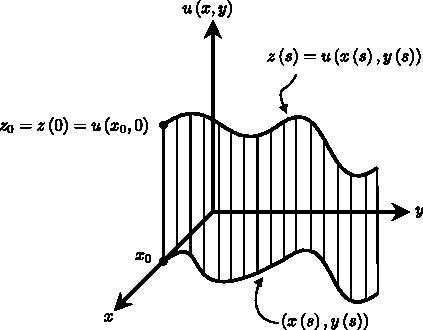
\includegraphics[width=0.35\paperwidth]{characteristics}
	\caption{The solution $u$ is described by the surface defined by
		$z=u\left(x,y\right)$.
		From any point $x_{0}$ on the $x$-axis, there is a curve
		$\left(x\left(s\right),y\left(s\right)\right)$ in the
		$xy$-plane, upon which wa can calculate the solution
		$z=u\left(x\left(s\right),y\left(s\right)\right)$.
		Knowing only the structure of the PDE, $x_{0}$ and $z_{0}$ we
		can solve ODEs to find the part of the solution surface which
		lies above the curve.}
\end{figure}

\begin{equation*}
	a\left(x,y\right)\diffp{u}{x}+
	b\left(x,y\right)\diffp{u}{y}=
	c_{1}\left(x,y\right)u+
	c_{2}\left(x,y\right),
	u\text{ given for }\left(x,y\right)\in\Gamma
\end{equation*}
where we have a linear PDE in the independent variables $x$ and $y$
with a given functions $a$, $b$, $c_{1}$ and $c_{2}$ of $\left(x,y\right)$.
$\Gamma\subset\partial\Omega$.
We find the characteristics, i.e., the curves which follow these directions, by solving
\begin{align*}
	\diff{x}{s}     & =
	a\left(x\left(s\right),y\left(s\right)\right). \\
	\diff{y}{s}     & =
	b\left(x\left(s\right),y\left(s\right)\right). \\
	z\left(s\right) & =
	u\left(x\left(s\right),y\left(s\right)\right).
\end{align*}

\begin{equation*}
	\diff{z}{s}=
	c_{1}\left(x\left(s\right),y\left(s\right)\right)
	z\left(s\right)+
	c_{2}\left(x\left(s\right),y\left(s\right)\right).
\end{equation*}

\chapter{Method of separation of variables}

% https://sci-hub.se/10.1137/S0895479801398025
